
%%%%%%%%%%%%%%%%%%%%%%%%%%%%%%%%%%%%%%%%%%%%%%%%%%%%%%%%%%%%%%%%%%%%%
%%%%%%%%%%%%%%%%%%%%%%%%%%%%%%%%%%%%%%%%%%%%%%%%%%%%%%%%%%%%%%%%%%%%%
%%%%%%%%%%%%%%%%%%%%%%%%%%%%%%%%%%%%%%%%%%%%%%%%%%%%%%%%%%%%%%%%%%%%%
%%%%%%%%%%%%%%%%%%%%%%%%%%%%%%%%%%%%%%%%%%%%%%%%%%%%%%%%%%%%%%%%%%%%%
\chapter{Choosing the technology}\label{kap:VyberTechnologie}
%%%%%%%%%%%%%%%%%%%%%%%%%%%%%%%%%%%%%%%%%%%%%%%%%%%%%%%%%%%%%%%%%%%%%
%%%%%%%%%%%%%%%%%%%%%%%%%%%%%%%%%%%%%%%%%%%%%%%%%%%%%%%%%%%%%%%%%%%%%
%%%%%%%%%%%%%%%%%%%%%%%%%%%%%%%%%%%%%%%%%%%%%%%%%%%%%%%%%%%%%%%%%%%%%
%%%%%%%%%%%%%%%%%%%%%%%%%%%%%%%%%%%%%%%%%%%%%%%%%%%%%%%%%%%%%%%%%%%%%

%%%%%%%%%%%%%%%%%%%%%%%%%%%%%%%%%%%%%%%%%%%%%%%%%%%%%%%%%%%%%%%%%%%%%
%%%%%%%%%%%%%%%%%%%%%%%%%%%%%%%%%%%%%%%%%%%%%%%%%%%%%%%%%%%%%%%%%%%%%
\section{Motivation}
%%%%%%%%%%%%%%%%%%%%%%%%%%%%%%%%%%%%%%%%%%%%%%%%%%%%%%%%%%%%%%%%%%%%%
%%%%%%%%%%%%%%%%%%%%%%%%%%%%%%%%%%%%%%%%%%%%%%%%%%%%%%%%%%%%%%%%%%%%%

One of the goals of this work is the utilization of open-source components.
We are going to combine several components and thus requiring access to their source code.
Many proprietary systems tend to push their proprietary protocols which hinders users from customization.

Some of the open standards concerning our effort are defined by the IETF\index{IETF}\footnote{Internet Engineering Task Force} organization which also defines important Internet standards. The standardization process within IETF is public in a form of RFC\index{RFC}\footnote{Request For Comments} documents which are collaboratively being developed by experts and the community. For the purposes of our thesis, we can use RFC as a source of standards for sound and video transmissions using the IP protocol.

Despite what we already said about proprietary systems, we could get inspired from the user experience and ergonomy of use point of view. Moreover, products such as VRVS \cite{VRVS-SK-Manual} or InSORS have already been founded on the infrastructure of existing open-source components (in this case the MBone tools). We could therefore easily reuse their approach in certain situations.

Last but not least, as stated in \cite{OpenMashProject}, we should be aware of the fact that the requirements of the scientific community will differ from the requirements of the commercial sector, some even being in conflict.

The rest of this chapter discusses the features of selected applications. The selection is based on personal preference of the author.

%%%%%%%%%%%%%%%%%%%%%%%%%%%%%%%%%%%%%%%%%%%%%%%%%%%%%%%%%%%%%%%%%%%%%%%%
%%%%%%%%%%%%%%%%%%%%%%%%%%%%%%%%%%%%%%%%%%%%%%%%%%%%%%%%%%%%%%%%%%%%%%%%
\section{Selected proprietary systems}
%%%%%%%%%%%%%%%%%%%%%%%%%%%%%%%%%%%%%%%%%%%%%%%%%%%%%%%%%%%%%%%%%%%%%%%%
%%%%%%%%%%%%%%%%%%%%%%%%%%%%%%%%%%%%%%%%%%%%%%%%%%%%%%%%%%%%%%%%%%%%%%%%

% ==================================
\subsection{Skype}\label{kap:Skype}
% ==================================
\begin{figure}
\centering
\includesvg[width=1\textwidth]{skype-architecture}
\caption{Overview of the Skype architecture.}
\label{fig:Skype-Architecture}
\end{figure}

Systém Skype sme vybrali ako zástupcu komerčne úspešného a masovo používaného systému s jednoduchou inštaláciou a obsluhou.

Obrázok \ref{fig:Skype-Architecture} znázorňuje spôsob komunikácie medzi uzlami v sieti Skype. Uzly umiestnené za sieťovým firewallom komunikujú s okolitým svetom prostredníctvom tzv. superuzlov\footnote{V ďalšom texte uvidíme ešte iné prístupy k riešeniu problémov spojených s firewallmi}. Prihlasovanie do siete sa uskutočňuje pomocou login servera. Po úspešnej autentifikácii sprostredkujú superuzly multimediálny prenos medzi koncovými klientmi. Nadväzovanie spojenia prebieha tak, že klient postupne kontaktuje najbližšie superuzly, ktoré rekurzívne kontaktujú svojich susedov až pokiaľ nie je známa trasa k volanému klientovi. Výsledné smerovanie multimediálnych paketov je zabezpečené na aplikačnej úrovni (podľa modelu ISO/OSI) a využíva sa decentralizovaná povaha siete Skype.

Spomínaná závislosť na superuzloch je priamo spojená s uzavretosťou protokolu Skype. Ako vidíme na obrázku \ref{fig:Skype-Architecture}, klient, ktorý disponuje dostatočne rýchlym pripojením a vlastnou IP adresou, sa mení na tzv. superuzol. Ako uvádza zdroj \cite{ArticleUreliable-Root-10-duvodu-proc-nepouzivat-skype}, pokiaľ by existovali alternatívne rozhrania, mohli by takéto aplikácie zabraňovať vzniku superuzlov, čo by sa následne odrazilo na celkovej kvalite prenosu v celej sieti Skype. Autori preto nemajú záujem na zverejňovaní svojho protokolu.

Automatický vznik superuzlov vedie k využívaniu prenosovej kapacity bez vedomia vlastníka siete. Problém sa prejaví pri spoplatnenom objeme prenesených dát, v Českej Republike napr. v sieti rozvodov káblovej televízie a internetu UPC alebo s pripojením ADSL.

\subsubsection*{Výhody}
\begin{paklist}
\item Jednoduchá inštalácia a obsluha.
\item Distribuovaná povaha aplikácie umožňuje prekonať NAT/firewall\index{NAT!traversal} pomocou siete superuzlov (obrázok \ref{fig:Skype-Architecture}).
\item Aplikácia je v súčasnosti zdarma, poskytovateľ umožňuje aj telefonické hovory do komerčných sietí.
\item Aplikácia je k dispozícii pre platformy Windows, Mac, Linux a Pocket PC.
\item Možnosť uskutočniť videokonferencie pomocou ďalších modulov -- text, audio, video, selektívne zdieľanie pracovnej plochy.
\item Komunikácia medzi uzlami je šifrovaná. Výmena kľúčov je zabezpečná pomocou 2048-bit RSA šifry a samotný prenos využíva 256-bit AES.
\end{paklist}

\subsubsection*{Neýhody}
\begin{paklist}
\item Uzavretý protokol.
\item Rozhranie pre platformu Linux zatiaľ vo verzii 1.3.0.53 neumožňuje prenos obrazu.
\item Vznik superuzlov, využívanie prenosovej kapacity bez vedomia vlastníka siete.
\item Aplikácia neumožňuje ovplyvňovať kvalitu prenosu priamo, nastavenie prebieha automaticky.
\item Systém nie je možné používať bez internetového pripojenia (napr. v izolovanej sieti LAN). Vždy je nutné kontaktovať Login server (obrázok \ref{fig:Skype-Architecture}).
\end{paklist}

% ==================================================
\subsection{Adobe Flash}\label{kap:Adobe Flash}
% ==================================================
Technológia Flash vzhľadom na svoje rozšírenie vo väčšine súčasných internetových prehliadačov môže ponúknuť spôsob ako dopraviť videokonferenčné riešenie k užívateľovi bez nutnosti inštalácie. Najnovšia verzia Flash 9 je dostupná pre platformy Windows, Mac a Linux, staršie verzie existujú pre platformy Solaris, HP-UX, BeOS a ďalšie. Ako príklad videokonferenčných riešení postavených na tejto technológii môžeme uviesť
InstantPresenter \cite{Company-Flash-InstantPresenter} alebo
FlashMeeting \cite{Company-Flash-FlashMeeting}.

\begin{figure}[htp]
\centering
\includesvg[width=0.6\textwidth]{flash-architecture}
%\includegraphics[width=0.45\textwidth]{images/app-flashmeeting-testtool}
%\includegraphics[width=0.45\textwidth]{images/app-flashmeeting-vote}
\caption{Architektúra Flash Media Server.}
\label{fig:Flash-Architecture}
\end{figure}

Na obrázku \ref{fig:Flash-Architecture} je znázornená centralizovaná povaha systému. Predpokladá sa, že centrálny prvok Flash Media Server disponuje verejnou IP adresou, a dostatočne rýchlym pripojením aby zvládla spracovať komunikáciu pripojených klientov (na obrázku označených ako "node"). Takto centralizovaná architektúra umožňuje prekonávať NAT/firewall\index{NAT!traversal}, pretože dokáže v krajnom prípade zabaliť komunikáciu do~TCP paketov.

Prenos multimediálnych paketov zabezpečuje proprietárny Real Time Messaging Protocol (RTMP\footnote{Nezamieňať s Routing Table Maintenance Protocolom z rodiny AppleTalk.}). Pretože neexistuje voľne dostupná špecifikácia RTMP, vznikol open-source projekt Red5 \cite{OpenSourceFlash-Red5}, ktorý pomocou reverse engineeringu\footnote{Autori označujú tento akt ako "discovery through observation".} implementuje jeho podstatnú časť \cite{OpenSourceFlash-RTMP-AMF}.
Protokol RTMP využíva UDP port 1935 a v prípade blokovania tunel cez TCP port 80 (HTTP).

\subsubsection*{Výhody}
\begin{paklist}
\item Technológia dostupná pre rôzne platformy.
\item Pokiaľ odhliadneme od nutnosti inštalovať samotný internetový prehliadač a flash-plugin, nevyžadujú ďalšie aplikácie žiadnu inštaláciu. Komunikácia prebieha priamo z internetového prehliadača.
\item Jednoduché nastavenie a kalibrácia kamery a mikrofónu.
\item Ďalšie vlastnosti, ktoré uvádza výrobca, ako napr. komunikácia cez SSL, vyvažovanie záťaže, QoS.
\item Množstvo open-source projektov súvisiacich s technológiou flash \cite{OpenSourceFlash-AllProjects}.
\end{paklist}

\subsubsection*{Neýhody}
\begin{paklist}
\item Systém je určený pre relatívne malé konferencie vzhľadom na vyššie hardwarové nároky samotnéhu flash-pluginu v porovnaní napr. s VRVS alebo AccessGridom popisovaných neskôr v tomto texte.
\item Zatiaľ neexistuje plnohodnotná open-source implementácia ani iná natívna implementácia pre architektúry x86-64, PowerPC, ARM.
\item Závislosť na reverse engineeringu.
\end{paklist}

% ==================================
\subsection{InSORS}\label{kap:InSORS}
% ==================================
Riešenie InSORS IG2 je postavené na technológii MBone o ktorej budeme hovoriť v ďalších kapitolách v súvislosti s AccessGridom (kapitola  \ref{kap:AccessGrid}). InSORS prináša integrované prostredie, ktoré zahŕňa softwarové aj hardwarové komponenty. Zákazník tak môže získať vyladený videokonferenčný systém, ktorý je ale zatiaľ dostupný iba pre platformu Windows.

\begin{figure}[htp]
\centering
\includesvg[width=0.8\textwidth]{arch-multicast}
\caption{Architektúra systému s použitím multicastovej siete.}
\label{fig:ArchMulticast}
\end{figure}

Podobne ako v prípade AccessGridu, prebieha komunikácia buď prostredníctvom multicastovej siete, alebo pomocou premostení z unicastovej siete (obrázok \ref{fig:ArchMulticast}).

Systém disponuje nástrojom IG Recorder, ktorý umožňuje okrem zvuku a obrazu nahrávať zdieľané prezentácie. Záznamy z konferencií je možné zároveň prehrať v~prebiehajúcej videokonferencií.

\subsubsection*{Výhody}
\begin{paklist}
\item Nahrávanie zdieľaných konferencií a prezentácií.
\item Integrované prostredie -- možnosť zakúpiť zároveň software aj hardware.
\item Integrácia s ostatnými VoIP technológiami, premostenie systémov H.323 a AccessGrid.
\item InSORS využíva otvorené štandardy ako napr. kodeky
H.261, H.263, H.264 (kapitoly \ref{kap:H.261}, \ref{kap:H.263}, \ref{kap:H.264}). Prenos multimediálnych dát je riešený pomocou protokolu RTP (kapitola \ref{kap:RTP+RTCP}).
\end{paklist}

\subsubsection*{Neýhody}
\begin{paklist}
\item Aplikácia je k dispozícii jedine pre platformu Windows.
\item Videokonferencia pomocou InSORS je spoplatnená.
\end{paklist}

% ==================================
\subsection{VRVS + EVO}\label{kap:VRVS}\index{VRVS!system}
% ==================================
Posledným zástupcom komerčných videokonferenčných riešení, ktorý v tejto práci popíšeme, je Virtual Rooms Videoconferencing Systems (VRVS) a jeho následník EVO. VRVS je distribuovaný systém určený pre komunikáciu v reálnom čase prístupný cez webové užívateľské rozhranie, ktoré využíva platformovo závislé aplikácie na strane klienta. Ide o upravené verzie MBone nástrojov akými sú napr. VIC (kapitola \ref{kap:VIC}) a RAT (kapitola \ref{kap:RAT}) z projektu OpenMash (kapitola \ref{kap:OpenMash}). Ďalšie komponenty, ako napr. premostenia pre softwarové alebo hardwarové H.323 klienty, používajú technológiu Java.

\begin{figure}[htp]
\centering
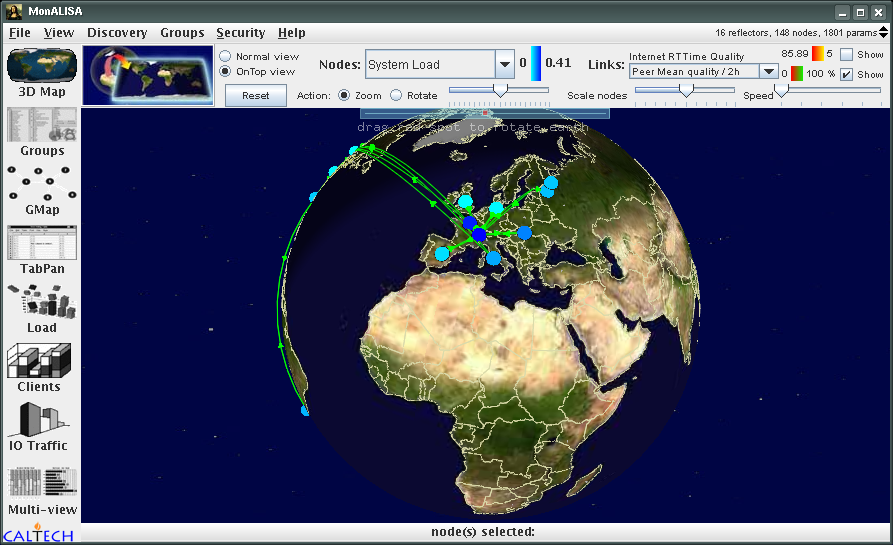
\includegraphics[width=0.48\textwidth]{images/app-monalisa1.png}
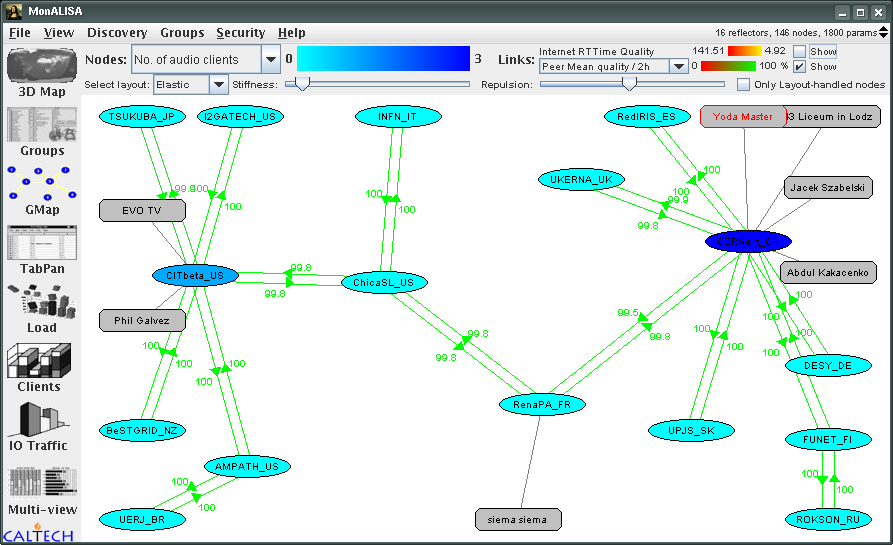
\includegraphics[width=0.48\textwidth]{images/app-monalisa3.png}
\caption{Monitorovanie distribuovaného systému VRVS reflektorov\index{VRVS!reflektor} pomocou aplikácie MonaLisa.}
\label{fig:MonaLisa-frontend}
\end{figure}

VRVS disponuje sieťou reflektorov\index{VRVS!reflektor} -- serverov rozmiestnených na rôznych miestach sveta, ktoré sprostredkovávajú komunikáciu medzi VRVS klientmi. Špeciálnym prípadom takéhoto reflektoru je VRVS-AG Reflector, ktorý umožňuje komunikovať s uzlami AccessGridu. Nezáleží, či klient disponuje unicast alebo multicast pripojením, VRVS transparentne premosťuje technológie AccessGrid, QuickTime a H.323.

Monitorovanie stavu VRVS\index{VRVS!monitoring} siete umožňuje upravená verzia systému MonaLisa\footnote{Moitoring Agents using a Large Integrated Services Architecture}. Jeho grafické rozhranie vidíme na obrázku \ref{fig:MonaLisa-frontend}. Vľavo je na svetovej mape znázornená sieť reflektorov umiestnených v Európe, vpravo je tá istá sieť znázornená vo~forme prehľadného grafu.

Zaujímavou funkciou, ktorá minimalizuje nároky na prenosovú kapacitu, je funkcia "Voice Switched mode". Autori VRVSV uvádzajú v publikácii \cite{VRVS-SK-Manual} nasledujúci príklad:

\begin{quote}
Príklad: Garantovaná kapacita siete je 1024Kbit/s. Videokonferencie sa zúčastňuje 15 partnerov. Každý vysiela kvalitný obraz (s datovými tokmi okolo 800Kbit/s). Kapacita siete by teda mala byť aspoň 12Mbit/s:

Počet účastníkov x 800 Kbit/s + 64Kbit/s (minimálny audio tok) =
= (15 x 800 + 64) Kbit/s = \textbf{12064Kbit/s}.

Riešenie: Použijeme „Voice Switched“ mode, takže vytvoríme požiadavku na VRVS reflektor\index{VRVS!reflektor}, aby posielal len video tok od toho partnera, ktorý práve rozpráva. Splnením tejto požiadavky dosiahneme obmedzenie toku na úroveň:

1 x 800Kbit/s (video) + 64Kbit/s (audio) = \textbf{864Kbit/s}.
\end{quote} 

Podobne ako InSORS a AccessGrid, podporuje VRVS aj nahrávanie konferencií. To však prebieha na strane servera, kde poverený operátor manuálne ovláda nahrávanie RTP paketov z vybranej virtuálnej miestnosti.

Aj keď ide o komerčný projekt California Institute of Technology, je systém dostupný zdarma pre vedeckú komunitu. Rozširovanie siete VRVS reflektorov\index{VRVS!reflektor} je spravované autormi systému. Po splnení kritérií môže záujemca poskytovať svoj vlastný reflektor pripojený do VRVS siete.
Užívatelia sú združení do skupín podľa oblasti záujmu, tzv. VRVS komunity (Internet2, SLOVAKIA\ldots)

V septembri 2003, bola otvorená Slovenská akademická videokonferenčná sieť, ktorá je k dispozícií všetkým univerzitám, výskumným ústavom SAV a vládnym organizáciám pripojených na optickú sieť SANET (Association of users of Slovak Academic data NETwork). Vznikol tak priestor pre experimentálne projekty ako napr. otvorené alebo dištančné vzdelávanie.

Nasledovníkom VRVS sa má v blízkej budúcnosti stať aplikácia EVO. Rozhranie je vytvorené v Jave a oproti VRVS podporuje navyše: Instant Messaging, Private Meetings (videokonferencia bez virtuálnej miestnosti), kryptovanie textových správ, výmenu súborov atď. Aplikácia je tiež multiplatformná.

\begin{samepage}
\subsubsection*{Výhody}
\begin{paklist}
\item Dostupnosť priamo z webového rozhrania -- automatická inštalácia.
\item Integrovaný systém rezervácie virtuálnych miestností.
\item P2P-sieť reflektorov.
\item Premostenie rozdielnych technológií.
\item Monitorovanie stavu siete.
\item Voice Switched mode.
\end{paklist}
\end{samepage}

\subsubsection*{Neýhody}
\begin{paklist}
\item Nutná výstavba siete reflektorov.
\item Užívateľ musí inštalovať Javu, potvrdzovať certifikáty.
\end{paklist}


%%%%%%%%%%%%%%%%%%%%%%%%%%%%%%%%%%%%%%%%%%%%%%%%%%%%%%%%%%%%%%%%%%%%%%%%%
%%%%%%%%%%%%%%%%%%%%%%%%%%%%%%%%%%%%%%%%%%%%%%%%%%%%%%%%%%%%%%%%%%%%%%%%%
\section{Vybrané voľne dostupné systémy}
%%%%%%%%%%%%%%%%%%%%%%%%%%%%%%%%%%%%%%%%%%%%%%%%%%%%%%%%%%%%%%%%%%%%%%%%%
%%%%%%%%%%%%%%%%%%%%%%%%%%%%%%%%%%%%%%%%%%%%%%%%%%%%%%%%%%%%%%%%%%%%%%%%%

% ================================================================
\subsection{VoIP riešenia}\label{kap:VoIP-Software}
% ================================================================
Z tejto kategórie vyberieme nasledujúce aplikácie: \textbf{Linphone}, \textbf{Ekiga}, \textbf{Wengophone} a \textbf{Asterisk}. Všetky existujú pre plaformy Windows aj Linux, sú dostupné pod licenciou GPL\footnote{General Public License $\Rightarrow$ open-source}, podporujú protokol SIP, prípadne H.323 (kapitola \ref{kap:VoIP-Protocols}).

Aplikácia Linphone umožňuje iba prenos zvuku. Ekiga a Wengophone využívajú pripojenú webkameru na prenos obrazu. Navyše poskytujú pre nových užívateľov bezplatný SIP účet \url{username@ekiga.net} resp. \url{username@voip.wengo.fr}. Wengophone dokonca poskytuje kredit pre volanie do pevnej a mobilnej telefónnej siete, prípadne prepája hovory priamo na SIP účet. Podporuje aj posielanie SMS správ.

Prenos obrazu je v oboch aplikáciách vo veľkosti CIF (obrázok \ref{fig:Resolutions}), každý uzol môže odosielať iba jeden obrazový a jeden zvukový dátový tok, čo znevýhodňuje nasadenie týchto aplikácií pre účely rozsiahlej videokonferencie, naopak postačuje pre účely desktop-to-desktop komunikácie.

Okrem SIP a H.323 klientov by sme radi spomenuli software určený pre chod telefónej ústredne (PBX). Asterisk podporuje prenos zvuku pomocou niekoľkých protoklov (IAX2, SIP, H.323), voicemail, adresárové služby, konferenčné hovory, odkazovač, prijímanie spojení čakajúcich vo fronte a ďalšie \ldots. Design protokolu IAX2 umožňuje prekonávať problémy s NAT/firewallmi\index{NAT!traversal}. Protokol SIP tiež podporuje preposielanie multimediálnych paketov cez tzv. STUN proxy server (napr. stun.ekiga.net). Nie je však natoľko úspešný ako práve IAX2.

\subsubsection*{Výhody}
\begin{paklist}
\item Existencia pre rôzne platformy, open-source, SIP je IETF štandard. IAX2 je vo fáze návrhu (IETF Internet-Draft \cite{IETFDraft-IAX2}).
\item Jednoduchá inštalácia a používanie.
\item Design IAX2 a STUN server pre SIP riešia problémy s NAT/firewallom.
\item Integrácia s telefónnymi linkami.
\item Kvalitné a efektívne kodeky ako napr. Speex.
\item Vstavané odstaňovanie spätnej väzby.
\item Pre Asterisk existuje špeciálna distribúcia Linuxu, dokonca aj vo formáte VMWare appliance.
\end{paklist}

\subsubsection*{Neýhody}
\begin{paklist}
\item Riešenia primárne určené pre telefonovanie.
\item Fixná veľkosť obrazu CIF a fixný počet dátových tokov obmedzuje použitie na desktop-to-desktop komunikáciu. Je to však problém konkrétnej implementácie, nie architektúry.
\item Kombinácia rôznych SIP klientov častokrát vedie k chybám pri spojovaní a komunikácii -- voľba nesprávneho kodeku, rozdielne implementácie protokolov.
\end{paklist}


% ============================================
\subsection{AccessGrid}\label{kap:AccessGrid}
% ============================================

Cieľom projektu AccessGrid (AG) je umožniť čo najprirodzenejšiu interakciu medzi účastníkmi konferencie s využitím existujúcej sieťovej infraštruktúry. Tento robustný nástoj pozostáva zo sady softwarových a hardwarových komponentov škálovateľných na mieru potrebám videokonferencie, od komunikácie medzi jednotlivcami až po celé skupiny.

Po softwarovej stránke tu môžeme nájsť komponenty určené na prenos obrazu, zvuku, zdieľanie prezentácií, vizualizačné a riadiace programy. Pre konferenciu prostredníctvom AG je obvykle vyhradená špeciálna miestnosť, čo umožňuje zabezpečiť kvalitnú komunikáciu aj pri veľkom počte účastníkov. Technológia AG je priamo navrhnutá pre spoluprácu medzi skupinami vedcov, kde prezentácia a vizualizácia výsledkov výskumu vyžaduje viac projekčnej techniky, kamier, náročnejšie spracovánie zvuku, a teda aj väčšie množstvo výpočtovej techniky potrebnej pre kódovanie zvuku a obrazu.

Obvykle takúto miestnosť označujeme ako uzol AccessGridu (AG node). Obrázok \ref{fig:ArchAccessGridDefault} znázorňuje príklad typickej architektúry AG node. Hneď na prvý pohľad si môžeme všimnúť distribuovanú povahu celého systému. Na obrázku sú znázornené štyri oddelené počítače -- Display Computer, Video Capture Computer, Audio Capture Computer a Control Computer. Po softwarovej stránke je AG zložený z komponentov VenueServer, VenueClient, NodeManager, NodeService a Bridge. Venue server predstavuje virtuálnu miestosť, v ktorej sa nachádzajú účastníci konferencie. Obsahuje súbory určené pre stiahnutie zdieľanými aplikáciami. Na VenueServer sa klienti pripájajú pomocou svojich VenueClientov, kde sa každý účastník autentifikuje pomocou certifikátu\footnote{O certifikát musí účastník dopredu požiadať certifikačnú autoritu. K tomuto účelu slúži špeciálny nástroj pomenovaný "Certificate Request Tool". V prípade nutnosti je možné použiť anonymný certifikát.}. NodeManager umožňuje ovládať distribuované prvky systému, zapínať a vypínať streamovacie služby. To sa deje prostredníctvom NodeService -- služieb spájajúcich oddelený hardware do distribuovaného systému, ktorý komunikuje pomocou XML-RPC. Posledným komponentom je Bridge, ktorý je určený na spostredkovanie služby pre účastnikov bez multicastovej siete.

V porovnaní s ostatnými technológiami sa môže zdať AG ako príliš zložitý systém. Kvalitný zážitok z videokonferencie za účasti veľkého počtu osôb, však vyžaduje viac investícií do zariadenia miestnosti. Obraz je na~rozdiel od monitoru zobrazovaný na projekčné plátno niekoľkými projektormi.

\begin{figure}
\centering
\includesvg[width=0.95\textwidth]{arch-ag-default}
\caption{Typická architektúra AccessGridu. (zdroje \protect\cite{ArticleUVTMU-KomunikaceAGPoint}\cite{childers00})}
\label{fig:ArchAccessGridDefault}
\end{figure}

\subsubsection*{Výhody}
\begin{paklist}
\item Škálovateľné riešenie podľa veľkosti konferencie.
\item Množstvo zdieľaných aplikácií a iných nástrojov.
\item Vysoká kvalita obrazu a zvuku.
\item Možnosť prenosu prostredníctvom unicast aj multicast siete.
\item Multiplatformnosť: Linux, Windows, MacOS X, FreeBSD
\end{paklist}

\subsubsection*{Neýhody}
\begin{paklist}
\item Architektúra vyžaduje rýchle sieťové pripojenie.
\item Bežný užívateľ môže mať problémy pri inštalácii a nastavení AG.
\item Vyššie nároky na priestor a vyššie finančné náklady na nákup potrebného hardware.
\item Problémy s multicastovým pripojením.
\item Problémy s prekonávaním NAT\index{NAT!problem}.
\end{paklist}


%%%%%%%%%%%%%%%%%%%%%%%%%%%%%%%%%%%%%%%%%%%%%%%%%%%%%%%%%%%%%%%%%%%%%%%%%
%%%%%%%%%%%%%%%%%%%%%%%%%%%%%%%%%%%%%%%%%%%%%%%%%%%%%%%%%%%%%%%%%%%%%%%%%
\section{Požiadavky a parametre zvoleného riešenia}
%%%%%%%%%%%%%%%%%%%%%%%%%%%%%%%%%%%%%%%%%%%%%%%%%%%%%%%%%%%%%%%%%%%%%%%%%
%%%%%%%%%%%%%%%%%%%%%%%%%%%%%%%%%%%%%%%%%%%%%%%%%%%%%%%%%%%%%%%%%%%%%%%%%

Predchádzajúci výber aplikácií nebol náhodný. Z komerčných riešení sme vybrali Skype pre jeho masové rozšírenie v oblasti IP telefonie a jeho schopnosť prekonávať NAT/firewall\index{NAT!traversal} pomocou distribuovaného systému superuzlov.
Adobe Flash sme vybrali pre jeho dostupnosť vo väčšine internetových prehliadačov a jednoduchosť inštalácie.
InSORS nás oslovil spôsobom, ktorým využíva technológiu MBone a ďalšie otvorené štandardy, ktoré ponúka v ľahko ovládateľnom balíku s možnosťou zakúpenia spolu so špecializovaným hardwarom.
Systém VRVS je pre nás príkladom aplikácie spustiteľnej priamo z webu (teda bez nutnosti inštalácie) a príkladom distribuovanej siete reflektorov monitorovaných systémom MonaLisa (obrázok \ref{fig:MonaLisa-frontend}).
Z~nekomerčných aplikácií sme vybrali Wengophone a Ekigu ako zástupcov SIP a H.323 a AccessGrid ako zástupcu robustného open-source videokonferenčného riešenia.

Cieľom nasledujúceho textu je definovať zoznam požiadaviek, ktoré kladieme na~výsledný systém na základe skúseností z existujúcich videokonferencčných riešení. V skutočnosti nemusí existovať systém, ktorý by vyhovoval všetkým požiadavkom, stačí ak sa tomuto ideálu priblíži.

%====================================
\subsection{Základné požiadavky}
%====================================

%---------------------
\paragraph*{Škálovateľnosť:}
Architektúra videokonferenčného systému by mala byť dostatočne flexibilná na to, aby umožňovala zároveň komunikáciu medzi veľkým aj malým počtom účastníkov, tým sa otvoria možnosti nasadenia v organizáciách nezávisle na~ich veľkosti. Veľké organizácie budú mať možnosť nasadiť distribuovanú verziu systému, zatiaľ čo malé organizácie vystačia so základným nastavaním. Príliš zaťažený systém by mal byť jednoducho rozšíriteľný o nové hardwarové komponenty. Túto myšlienku by sme mohli rozvinúť až tak ďaleko, že budeme uvažovať o~vytvorení virtuálnej univerzity s množstvom simultánne prebiehajúcich prednášok.

%---------------------
\paragraph*{Bezpečnosť:}
Umožniť šifrovanú komunikáciu v~rámci konferencie. V ideálnom prípade úplné šifrovanie všetkých správ. Možnosť voľby miery zabezpečenia. Ďalšou funkčnosťou môže byť autentifikácia a autorizácia účastníkov tak, aby mali prístup do vybranej podmnožiny prebiehajúcich konferencií. V prípade bezpečnosti budeme taktiež požadovať, aby dátové prenosy nemohli byť modifikované neznámimi subjektmi (integrita).
Pre niektoré organizácie býva práve táto požiadavka kľúčová.

%---------------------
\paragraph*{Dostupnosť:}
Hlavne vyriešenie problémov spojených s firewallmi, NAT\index{NAT!požiadavka dostupnosti} a proxy servermi. Množstvo klientov sa nachádza za istou formou NAT kvôli problémom adresovania v IPv4 sieti. Sieť býva navyše obohatená o firewall, prípadne rôzne formy tzv. transparent proxy. Dokonalý prechod cez všetky sieťové prekážky by bol veľmi komplikovaný, ale systém by mal počítať aspoň s najbežnejšími problémami, hlavne NAT.

%---------------------
\paragraph*{Modifikovateľnosť:}
Možnosť zmeny komponentov systému.

%---------------------
\paragraph*{Stabilita:}
Stabilita v čase. Systém by mal byť schopný bežať nepretržite bez pádu. V prípade poruchy by mal zanechať konzistentnú množinu dát.

%---------------------
\paragraph*{Prenosová kapacita:}
Úspech videokonferencie výrazne závisí na rýchlosti siete, ktorou účastníci disponujú.

%---------------------
\paragraph*{One-way Latency:}\index{latency!one-way}
Jednosmerná reakčná odozva je doba medzi odoslaním paketu na strane odosielateľa a prijatím paketu na strane príjemcu. V ďalšom texte nás bude hlavne zaujímať hodnota Round-trip Latency.

%---------------------
\paragraph*{Round-trip Latency:}\index{latency!round-trip}
Túto veličinu definujeme ako dobu medzi odoslaním požiadavku a prijatím odpovede ($\approx 2 \times one way latency$). V texte ju budeme používať pod názvom \textbf{Reakčná odozva} resp. \textbf{Latency}. V literatúre \cite{ITU-G.114-One-way-transmission-time} sa uvádza, že v~prípade zvuku by nemala presahovať 300ms, inak si účastníci rozhovoru prestávajú rozumieť. Znázorňuje to aj obrázok \ref{fig:ITU-G.114}. V prípade prenosu obrazu môže byť táto hodnota bez problémov niekoľkonásobne väčšia. V multimediálnej komunikácii preto uprednostníme nespoľahlivé nepotvrdzované doručovanie tzv. \textbf{Unreliable Unicast/Multicast}. Doručovanie pomocou UDP pred TCP.

\begin{figure}
\centering
\includesvg[width=0.7\textwidth]{mouth-to-ear-delay}
\caption{Dôsledky oneskorenia zvuku podľa ITU-T G.114 \protect\cite{ITU-G.114-One-way-transmission-time}.}
\label{fig:ITU-G.114}
\end{figure}

%---------------------
\paragraph*{Jitter:}
Rozptyl reakčnej odozvy definujeme ako zmenu reakčnej odozvy v čase. Garancia maximálnej hodnoty pre jitter umožňuje odhadnúť veľkosti bufferov. Použitie bufferov je však obmedzené celkovou latenciou.

%---------------------
\paragraph*{Hardwarové nároky:}
Zamýšľaný systém bude spracovávať desiatky nezávislých dátových tokov. Použité kodeky musia byť v tom prípade nenáročné na výpočtový výkon. Hardwarovo náročné procesy môžu zhoršiť reakčnú odozvu systému. Tento problém sa týka hlavne spracovania obrazu.

%---------------------
\paragraph*{Štandardy:}
Budeme používať štandardizované komunikačné protokoly a kodeky. Táto požiadavka plynie už z nášho zámeru požívať jedine open-source software. Pre prenos multimediálnych paketov tak prichádza do úvahy protokol RTP (kapitola \ref{kap:RTP+RTCP}).

%---------------------
\paragraph*{Dostupnosť pre rôzne platformy:}
Umožniť sledovanie konferencie minimálne na systémoch Linux a Windows.

%=======================
\subsection{Obraz}
%=======================

%---------------------
\paragraph*{Veľkost obrazu:}
Systém by mal umožniť voľbu veľkostí obrazu. Myslíme tým hlavne rozdiely medzi snímaním veľkej miestnosti s množstvom účastníkov oproti detailnému snímaniu tváre. Predpokladáme, že jednotlivé obrazové toky budeme zobrazovať na veľké projekčné plátno pomocou data-projektora, preto doporučujeme použiť aspoň formát D1 PAL 720x576 (viď obrázok \ref{fig:Resolutions}). Implicitným formátom väčšiny súčasných videokonferenčných systémov býva totiž formát CIF 352x288 resp. 352x240 (viď obrázok \ref{fig:Resolutions}). Toto obmedzenie sa týka hlavne použitého kodeku H.261 (pozri kap. \ref{kap:H.261}).

% **********************************************
% Image Resolutions
% **********************************************
\begin{figure}
\centering
\includesvg[width=0.6\textwidth]{resolutions}
\caption{Porovnanie rôznych veľkostí obrazu.}
\label{fig:Resolutions}
\end{figure}
% **********************************************

Popisované systémy Skype a Flash
(kap. \ref{kap:Skype}, \ref{kap:Adobe Flash})
pracujú s fixnou veľkosťou obrazu.
Výhodou je jednoduchšia implementácia a ovládanie zo strany užívateľa.
Naopak systémy AccessGrid, InSORS a VRVS
(kap. \ref{kap:AccessGrid}, \ref{kap:InSORS}, \ref{kap:VRVS})
dávajú možnosť voľby na úkor jednoduchosti.

%---------------------
\paragraph*{Kódovanie pohybu:}
Obraz z miestnosti, kde prebieha konferencia, može mať statickú alebo dynamickú povahu, čo by sme mali zohľadniť aj pri voľbe vhodného kodeku. Za statický obraz v tomto prípade pokladáme napr. skupinu sediacich ľudí, ktorí sú snímaní kamerou z niekoľkometrovej vzdialenosti pri konštantných svetelných podmienkach. Príkladom dynamického obrazu môže byť napr. jedna osoba snímaná z blízka, prípadne množstvo pohyblivých objektov. Slabé osvetlenie navyše spôsobuje nárast dátového toku, pretože kamery pridávajú do obrazu rôzne artefakty.

%---------------------
\paragraph*{Kvalita obrazu:}
Pokiaľ nám ide o komunikáciu medzi jednotlivcami, ktorí navyše disponujú prenosovou kapacitou menšou ako 1Mbit/s, prirodzene nám postačí nižšia kvalita obrazu ako v prípade rozsiahlej konferencie, kde obvykle vyžadujeme aspoň 10 Mbit/s. V prípade požiadavku na prenosy vo vysokej kvalite musíme počítať dokonca s kapacitou 25Mbit/s pre jeden dátový tok (komprimované video vo formáte HDV). Rozpracovanie tejto problematiky je možné nájsť napr. v článku \cite{ArticleUVTMU-VideokonferenceSVysokouKvalitou}.

%=======================
\subsection{Zvuk}
%=======================

%---------------------
\paragraph*{Kvalita zvuku:}
Na kvalitu zvuku kladieme vyššie nároky než na kvalitu obrazu. Človek je oveľa citlivejší na drobné výpadky zvuku ako na úplnú absenciu obrazu. (V~kapitole \ref{kap:RTP+RTCP}, pojednávame o protokole RTP, ktorý práve z tohto dôvodu používa oddelené UDP porty pre prenos zvuku a obrazu).
Pokiaľ chceme prenášať reč a nezaujíma nás prenos hudby v najvyššej kvalite, vystačíme s frekvenciou okolo 8000Hz. Najväčším nepriateľom pre nás bude latency (reakčná odozva) resp. jitter (rozptyl reakčnej odozvy).

%---------------------
\paragraph*{Problém spätnej väzby:}
V podmienkach ozvučenej miestnosti sa musí systém vyrovnať so vznikom spätnej väzby a inými nevhodnými zvukovými efektmi. Potlačenie ozveny má vyššiu prioritu ako samotná kvalita zvukového signálu.

%==========================================
\subsection{Prezentácia/Vizualizácia}
%==========================================

%---------------------
\paragraph*{Podporované formáty:}
Od poskytovateľa videokonferenčnej technológie sa očakáva, že bude v~maximálnej miere vychádzať v ústrety účastníkom a podporovať široké portfólio formátov. V ideálnom prípade by účastníci nemali byť obmedzovaní pri výbere formátu, ktorý chcú prezentovať. V reálnom svete však musí poskytovateľ definovať zoznam podporovaných formátov a oboznámiť s ním všetkých zainteresovaných účastníkov s dostatočným predstihom.

%---------------------
\paragraph*{Video sekvencie:}
Mali by sme podporovať rôzne kodeky a veľkosti od súborov s desiatkami MiB až po video uložené vo formáte DVD. Typickým požiadavkom užívateľa môže byť spustenie video sekvenice, ktorú je možné ovládať minimálne tlačítkom PLAY/PAUSE.

Automatické konverzie medzi video formátmi zvládajú napr. nástroje FFMPEG, MPlayer a VLC. Zvukové súbory môžeme konvertovať pomocou nástroja sox. Pre interaktívnu úpravu zvuku je vhodná aplikácia Audacity, v prípade obrazu poslúži napr. Avidemux.

%---------------------
\paragraph*{Prezentácia vo forme statických snímkov:}
Obvyklým formátom pre prípravu prezentácie bývajú formáty PDF a PPT. V~našom riešení budeme uprednostňovať formát PDF. Účastníci videokonferencie budú totiž nútení vypustiť videosekvencie a animované prechody medzi snímkami zo svojich prezentácií. Zmenší sa tak objem prenesených dát aj záťaž procesoru.

Účastníci, ktorí inklinujú k prostrediu typu Unix budú pravdepodobne používať formáty PDF, PS (PostScript) alebo ODF (Open Document Format). Užívatelia Windows prinesú pravdepodobne formáty PPT, PDF alebo ODF. Automatickú konverziu je možné zabezpečiť jednoduchým skriptom, ktorý využíva OpenOffice makrojazyk (zdroj \cite{OpenOffice-Conversion})
Ďalšie úpravy vektorových formátov pokrývajú nástroje pstoedit, a2ping a xpdf. Automatické konverzie medzi rastrovými formátmi je možné zabezpečiť pomocou balíka NetPbm a ImageMagick. Pre vizualizáciu dát pomocou skriptov môžeme využiť programy Gnuplot, R či Graphviz.

%---------------------
\paragraph*{Interaktívne 2D/3D simulácie:}
Do tejto kategórie patria rôzne 3D modely a prostredia vytvorené v špecializovaných aplikáciách typu 3D Studio Max, Blender, SolidEdge či AutoCad. Patria sem aj prostredia vytvorené pre niektorý z herných enginov ako napr. Unreal, Half-Life, Quake a mnoho ďalších. Medzi prostredia, ktoré by sme mohli podporovať patrí ďalej OpenInventor a VRML.

\begin{samepage}
\noindent
Spôsoby prezentácie by sme mohli rozdeliť do štyroch skupín:
\begin{enumerate}
\item Programy spustené na externom počítači, ktorý je pripojený S-Video signálom.
\item Programy používajúce VNC display.
\item Programy, ktoré priamo podporujú kolaboráciu.
\item Programy emulované pomocou VMWare.
\end{enumerate}
\end{samepage}

\noindent
Počas videokonferencií Polylogues sa ukázalo, že najstabilnejším riešením je použitie externého počítača pripojeného cez S-Video. Užívateľ tak môže priniesť vlastné prostredie, na ktorom má odladenú svoju prezentáciu.

%---------------------
\paragraph*{Obraz z externého zdroja:}
Už sme spomenuli, že vhodným riešením je použiť externý hardware pripojený cez S-Video do digitalizačnej karty. Nevýhodou môže byť nutnosť zakúpenia ďalšieho hardwarového komponentu. Niekedy však užívateľ nedisponuje ani S-Video výstupom, takže musíme pristúpiť napr. k inštalácii VNC.

%---------------------
\paragraph*{Kvalita:}
Pri prenose videosekvencií spolu so zvukom platia rovnaké pravidlá ako sme stanovili v požiadavkoch na obraz a zvuk. Navyše musíme brať do úvahy, že pri prezentácii snímkov, ktoré majú väčšinou statickú povahu budeme používať iné techniky, kodeky, veľkosti obrazu. Situáciu mierne komplikujú prezentácie, ktoré v~sebe obsahujú videosekvencie. Z toho dôvodu uprednostňujeme prezentáciu vo~formáte PDF.

%---------------------
\paragraph*{Ovládanie:}
Účastníci konferencie by mali dostať možnosť ovládať prebiehajúcu prezentáciu. V prípade AccessGridu je to napr. SharedPresentation alebo SharedPDF.

%=======================
\subsection{Spolupráca}
%=======================

%http://www.vide.net/cookbook/cookbook.en/
%HighlightVideoConsumer, PositionalAudioService
%http://scv.bu.edu/~putnam/ag-audio/services-2.4/doc/

Riešenie by malo podporovať rôzne formy spolupráce medzi účastníkmi konferencie. Od jednoduchého zdieľania súborov až po zdieľanú pracovnú plochu. V tomto prípade môžeme znova využiť vlastnosti VNC.

%%%%%%%%%%%%%%%%%%%%%%%%%%%%%%%%%%%%%%%%%%%%%%%%%%%%%%%%%%%%%%%%%%%%%
%%%%%%%%%%%%%%%%%%%%%%%%%%%%%%%%%%%%%%%%%%%%%%%%%%%%%%%%%%%%%%%%%%%%%
\section{Vybraný systém}
%%%%%%%%%%%%%%%%%%%%%%%%%%%%%%%%%%%%%%%%%%%%%%%%%%%%%%%%%%%%%%%%%%%%%
%%%%%%%%%%%%%%%%%%%%%%%%%%%%%%%%%%%%%%%%%%%%%%%%%%%%%%%%%%%%%%%%%%%%%

V prvej kapitole sme popísali niekoľko existujúcich aplikácií, vyberali sme hlavne prakticky odskúšané riešenia z oblasti closed-source aj open-source software. Snažili sme sa popísať technológie vhodné pre desktop-to-desktop komunikáciu ako aj pre group-to-group komunikáciu a poukázali sme na rozdiely medzi oboma prístupmi. Pre každú aplikáciu sme pripravili zoznam ich výhod a nevýhod. Vytvorili sme obraz ideálneho videokonferenčného systému tak, že sme poskytli detailný zoznam požiadaviek. To nám umožní vybrať vhodné protokoly, kodeky a komponenty. Z~voľne dostupných technológií vyberáme AccessGrid, pretože vo svete open-source sa jedná o najkomplexnejší videokonferenčný systém, ktorého základ využívajú aj niektoré komerčné produkty.
